\chapter{Mammalian Anatomy II}\label{mammalian-anatomy-ii}

\section{Skin}\label{skin}

\href{https://en.wikipedia.org/wiki/Skin}{Skin} is the soft outer tissue
covering vertebrates. Other animal coverings, such as the arthropod
exoskeleton, have different developmental origin, structure and chemical
composition. The adjective cutaneous means ``of the skin'' (from Latin
cutis, skin). In mammals, the skin is an organ of the integumentary
system made up of multiple layers of ectodermal tissue, and guards the
underlying muscles, bones, ligaments and internal organs. Skin of a
different nature exists in amphibians, reptiles, and birds. All mammals
have some hair on their skin, even marine mammals like whales, dolphins,
and porpoises which appear to be hairless. The skin interfaces with the
environment and is the first line of defense from external factors. For
example, the skin plays a key role in protecting the body against
pathogens and excessive water loss. Its other functions are insulation,
temperature regulation, sensation, and the production of vitamin D
folates. Severely damaged skin may heal by forming scar tissue. This is
sometimes discolored and depigmented. The thickness of skin also varies
from location to location on an organism. In humans for example, the
skin located under the eyes and around the eyelids is the thinnest skin
in the body at 0.5 mm thick, and is one of the first areas to show signs
of aging such as ``crows feet'' and wrinkles. The skin on the palms and
the soles of the feet is 4 mm thick and is the thickest skin on the
body.

\href{https://en.wikipedia.org/wiki/Fur}{Fur} is the hair covering of
non-human mammals, particularly those mammals with extensive body hair
that is soft and thick. Primarily, fur augments the insulation the skin
provides but can also serve as a secondary sexual characteristic or as
camouflage. On some animals, the skin is very hard and thick, and can be
processed to create leather. Reptiles and fish have hard protective
scales on their skin for protection, and birds have hard feathers, all
made of tough β-keratins. Amphibian skin is not a strong barrier,
especially regarding the passage of chemicals via skin and is often
subject to osmosis and diffusive forces. For example, a frog sitting in
an anesthetic solution would be sedated quickly, as the chemical
diffuses through its skin. Amphibian skin plays key roles in everyday
survival and their ability to exploit a wide range of habitats and
ecological conditions.

Mammalian skin is composed of two primary layers:

\begin{itemize}
\tightlist
\item
  the epidermis, which provides waterproofing and serves as a barrier to
  infection; and
\item
  the dermis, which serves as a location for the appendages of skin;
\end{itemize}

\begin{figure}

{\centering 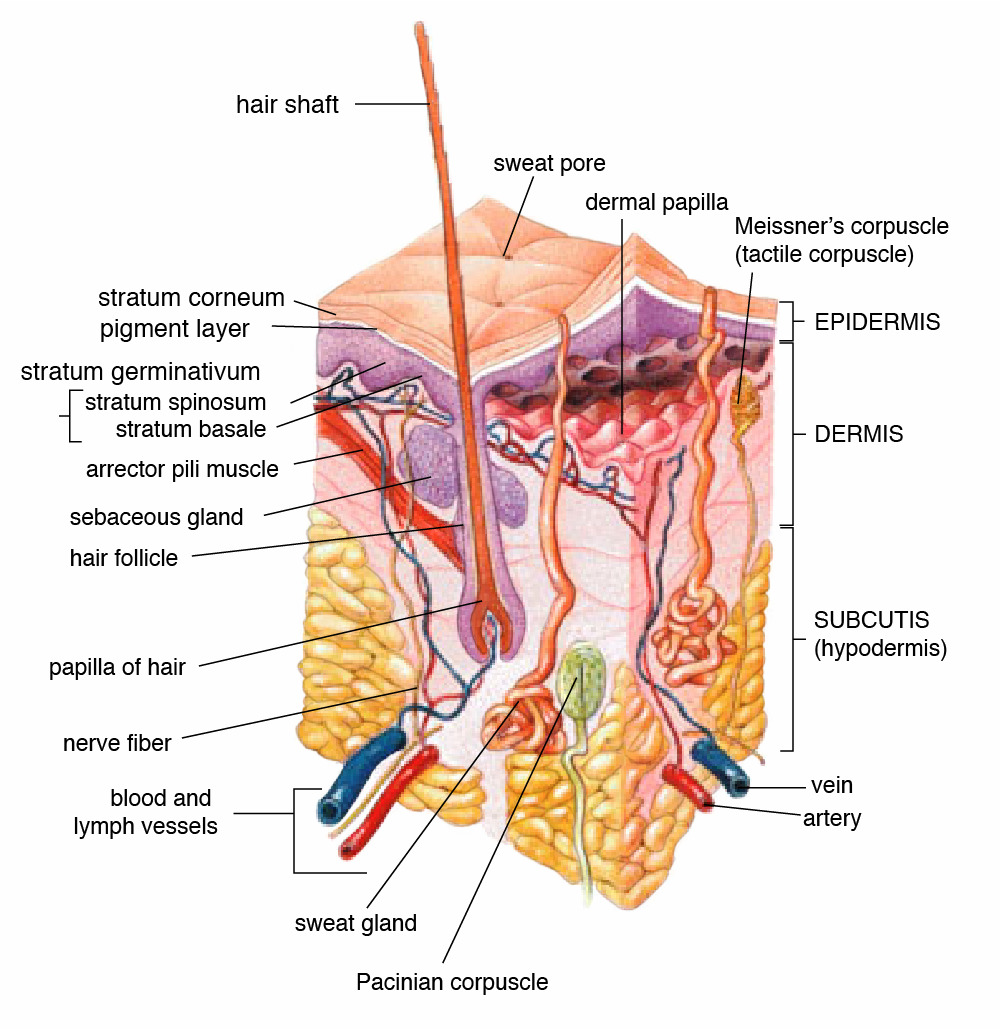
\includegraphics[width=0.7\linewidth]{./figures/anatomy/skin}

}

\caption{\href{https://commons.wikimedia.org/wiki/File:Skin.png}{Anatomy of human
skin.}}\label{fig:skin}
\end{figure}

\section{Epidermis}\label{epidermis}

The \href{https://en.wikipedia.org/wiki/Epidermis}{epidermis} is
composed of the outermost layers of the skin. It forms a protective
barrier over the body's surface, responsible for keeping water in the
body and preventing pathogens from entering, and is a stratified
squamous epithelium, composed of proliferating basal and differentiated
suprabasal keratinocytes.

Keratinocytes are the major cells, constituting 95\% of the epidermis,
while Merkel cells, melanocytes and Langerhans cells are also present.
The epidermis can be further subdivided into the following strata or
layers (beginning with the outermost layer):

\begin{itemize}
\tightlist
\item
  Stratum corneum
\item
  Stratum lucidum (only in palms and soles)
\item
  Stratum granulosum
\item
  Stratum spinosum
\item
  Stratum germinativum (also called the stratum basale)
\end{itemize}

Keratinocytes in the stratum basale proliferate through mitosis and the
daughter cells move up the strata changing shape and composition as they
undergo multiple stages of cell differentiation to eventually loose
their nuclei. During that process, keratinocytes will become highly
organized, forming cellular junctions (desmosomes) between each other
and secreting keratin proteins and lipids which contribute to the
formation of an extracellular matrix and provide mechanical strength to
the skin. Keratinocytes from the stratum corneum are eventually shed
from the surface (desquamation).

The epidermis contains no blood vessels, and cells in the deepest layers
are nourished by diffusion from blood capillaries extending to the upper
layers of the dermis.

\section{Basement membrane}\label{basement-membrane}

The epidermis and dermis are separated by a thin sheet of fibers called
the basement membrane, and is made through the action of both tissues.
The basement membrane controls the traffic of the cells and molecules
between the dermis and epidermis but also serves, through the binding of
a variety of cytokines and growth factors, as a reservoir for their
controlled release during physiological remodeling or repair processes.

\section{Dermis}\label{dermis}

The \href{https://en.wikipedia.org/wiki/Dermis}{dermis} is the layer of
skin beneath the epidermis that consists of connective tissue and
cushions the body from stress and strain. The dermis provides tensile
strength and elasticity to the skin through an extracellular matrix
composed of collagen fibrils, microfibrils, and elastic fibers, embedded
in hyaluronan and proteoglycans.

It harbors many mechanoreceptors (nerve endings) that provide the sense
of touch and heat through nociceptors and thermoreceptors. It also
contains the hair follicles, sweat glands, sebaceous glands, apocrine
glands, lymphatic vessels and blood vessels. The blood vessels in the
dermis provide nourishment and waste removal from its own cells as well
as for the epidermis.

The dermis is tightly connected to the epidermis through a basement
membrane and is structurally divided into two areas: a superficial area
adjacent to the epidermis, called the papillary region, and a deep
thicker area known as the reticular region.

\section{Papillary region}\label{papillary-region}

The papillary region is composed of loose areolar connective tissue.This
is named for its fingerlike projections called papillae that extend
toward the epidermis. The papillae provide the dermis with a ``bumpy''
surface that interdigitates with the epidermis, strengthening the
connection between the two layers of skin.

\section{Reticular region}\label{reticular-region}

The reticular region lies deep in the papillary region and is usually
much thicker. It is composed of dense irregular connective tissue, and
receives its name from the dense concentration of collagenous, elastic,
and reticular fibers that weave throughout it. These protein fibers give
the dermis its properties of strength, extensibility, and elasticity.
Also located within the reticular region are the roots of the hair,
sweat glands, sebaceous glands receptors, nails, and blood vessels.

\section{Subcutaneous tissue}\label{subcutaneous-tissue}

The subcutaneous tissue (also hypodermis) is not part of the skin, and
lies below the dermis. Its purpose is to attach the skin to underlying
bone and muscle as well as supplying it with blood vessels and nerves.
It consists of loose connective tissue and elastin. The main cell types
are fibroblasts, macrophages and adipocytes (the subcutaneous tissue
contains 50\% of body fat). Fat serves as padding and insulation for the
body.

Microorganisms like \emph{Staphylococcus epidermidis} colonize the skin
surface. The density of skin flora depends on region of the skin. The
disinfected skin surface gets recolonized from bacteria residing in the
deeper areas of the hair follicle, gut and urogenital openings.

\section{Muscle}\label{muscle}

\href{https://en.wikipedia.org/wiki/Muscle}{Muscle} is a soft tissue
found in most animals. Muscle cells contain protein filaments of actin
and myosin that slide past one another, producing a contraction that
changes both the length and the shape of the cell. Muscles function to
produce force and motion. They are primarily responsible for maintaining
and changing posture, locomotion, as well as movement of internal
organs, such as the contraction of the heart and the movement of food
through the digestive system via peristalsis.

Muscle tissues are derived from the mesodermal layer of embryonic germ
cells in a process known as myogenesis. There are three types of muscle,
skeletal or striated, cardiac, and smooth. Muscle action can be
classified as being either voluntary or involuntary. Cardiac and smooth
muscles contract without conscious thought and are termed involuntary,
whereas the skeletal muscles contract upon command.

The term muscle is derived from the Latin musculus meaning ``little
mouse'' perhaps because of the shape of certain muscles or because
contracting muscles look like mice moving under the skin.

The muscular system consists of all the muscles present in a single
body. There are approximately 650 skeletal muscles in the human body,
but an exact number is difficult to define. The difficulty lies partly
in the fact that different sources group the muscles differently and
partly in that some muscles, such as palmaris longus, are not always
present.

The muscular system is one component of the musculoskeletal system,
which includes not only the muscles but also the bones, joints, tendons,
and other structures that permit movement.

\section{Cartilage}\label{cartilage}

\href{https://en.wikipedia.org/wiki/Cartilage}{Cartilage} is a resilient
and smooth elastic tissue, rubber-like padding that covers and protects
the ends of long bones at the joints, and is a structural component of
the rib cage, the ear, the nose, the bronchial tubes, the intervertebral
discs, and many other body components. It is not as hard and rigid as
bone, but it is much stiffer and much less flexible than muscle.

Because of its rigidity, cartilage often serves the purpose of holding
tubes open in the body. Examples include the rings of the trachea, such
as the cricoid cartilage and carina.

Cartilage is composed of specialized cells called chondrocytes that
produce a large amount of collagenous extracellular matrix, abundant
ground substance that is rich in proteoglycan and elastin fibers.
Cartilage is classified in three types, elastic cartilage (Figure
\ref{fig:elastic}), hyaline cartilage (Figure \ref{fig:hyaline}) and
fibrocartilage (Figure \ref{fig:fibro}), which differ in relative
amounts of collagen and proteoglycan.

Cartilage does not contain blood vessels (it is avascular) or nerves (it
is aneural). Nutrition is supplied to the chondrocytes by diffusion. The
compression of the articular cartilage or flexion of the elastic
cartilage generates fluid flow, which assists diffusion of nutrients to
the chondrocytes. Compared to other connective tissues, cartilage has a
very slow turnover of its extracellular matrix and does not repair.

\section{Bone}\label{bone}

\href{https://en.wikipedia.org/wiki/Bone}{Bones} support and protect the
various organs of the body, produce red and white blood cells, store
minerals, provide structure and support for the body, and enable
mobility. Bones come in a variety of shapes and sizes and have a complex
internal and external structure. They are lightweight yet strong and
hard, and serve multiple functions.

Bone tissue (osseous tissue) is a hard tissue, a type of dense
connective tissue. It has a honeycomb-like matrix internally, which
helps to give the bone rigidity. Bone tissue is made up of different
types of bone cells. Osteoblasts and osteocytes are involved in the
formation and mineralization of bone; osteoclasts are involved in the
resorption of bone tissue. Modified (flattened) osteoblasts become the
lining cells that form a protective layer on the bone surface. The
mineralized matrix of bone tissue has an organic component of mainly
collagen called ossein and an inorganic component of bone mineral made
up of various salts. Bone tissue is a mineralized tissue of two types,
cortical bone and cancellous bone. Other types of tissue found in bones
include bone marrow, endosteum, periosteum, nerves, blood vessels and
cartilage.

In the human body at birth, there are over 270 bones but many of these
fuse together during development, leaving a total of 206 separate bones
in the adult, not counting numerous small sesamoid bones. The largest
bone in the body is the femur or thigh-bone, and the smallest is the
stapes in the middle ear.

The Latin word for bone is os, hence the many terms that use it as a
prefix -- such as osseous and osteopathy.

Bone is not uniformly solid, but includes a tough matrix. This matrix
makes up about 30\% of the bone and the other 70\% is of salts that give
strength to it. The matrix is made up of between 90 and 95\% collagen
fibers, and the remainder is ground substance. The primary tissue of
bone, bone tissue (osseous tissue), is relatively hard and lightweight.
Its matrix is mostly made up of a composite material incorporating the
inorganic mineral calcium phosphate in the chemical arrangement termed
calcium hydroxylapatite (this is the bone mineral that gives bones their
rigidity) and collagen, an elastic protein which improves fracture
resistance. The collagen of bone is known as ossein. Bone is formed by
the hardening of this matrix around entrapped cells. When these cells
become entrapped from osteoblasts they become osteocytes.

The hard, outer layer of bones is composed of cortical bone also called
compact bone being much denser than cancellous bone. It forms the hard
exterior (cortex) of bones. The cortical bone gives bone its smooth,
white, and solid appearance. It facilitates bone's main functions: to
support the whole body, protect organs, provide levers for movement, and
store and release chemical elements, mainly calcium. It consists of
multiple microscopic columns, each called an osteon. Each column is
multiple layers of osteoblasts and osteocytes around a central canal
called the Haversian canal. Volkmann's canals at right angles connect
the osteons together. The columns are metabolically active, and as bone
is reabsorbed and created the nature and location of the cells within
the osteon will change. Cortical bone is covered by a periosteum on its
outer surface, and an endosteum on its inner surface. The endosteum is
the boundary between the cortical bone and the cancellous bone. The
primary anatomical and functional unit of cortical bone is the osteon.

Spongy bone tissue is the internal tissue of the skeletal bone and is an
open cell porous network. Spongy bone is typically found at the ends of
long bones, near to joints and within the interior of vertebrae. Spongy
bone is highly vascular and frequently contains red bone marrow where
hematopoiesis, the production of blood cells, occurs. The primary
anatomical and functional unit of spongy bone is the trabecula. The
trabeculae are aligned towards the mechanical load distribution that a
bone experiences within long bones such as the femur. Within these
spaces are bone marrow and hematopoietic stem cells that give rise to
platelets, red blood cells and white blood cells.

\begin{figure}

{\centering 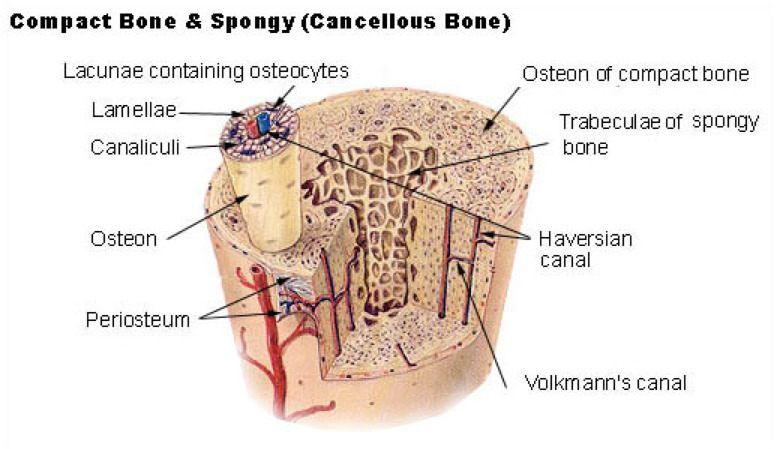
\includegraphics[width=0.7\linewidth]{./figures/anatomy/bone}

}

\caption{\href{https://commons.wikimedia.org/wiki/File:Illu_compact_spongy_bone.jpg}{Compact
and spongy bone.}}\label{fig:bone}
\end{figure}

\section{The Kidneys}\label{the-kidneys}

The \href{https://en.wikipedia.org/wiki/Kidney}{kidneys} are two
bean-shaped organs found on the left and right sides of the body in
vertebrates. They are located at the back of the abdominal cavity in the
retroperitoneal space. In adult humans, they are about 11 centimeters in
length. They receive blood from the paired renal arteries; blood exits
into the paired renal veins. Each kidney is attached to a ureter, a tube
that carries excreted urine to the bladder.

The nephron is the structural and functional unit of the kidney. Each
adult kidney contains around one million nephrons. The nephron utilizes
four processes to alter the blood plasma which flows to it: filtration,
reabsorption, secretion, and excretion. Via one or more of these
mechanisms, the kidney participates in the control of the volume of
various body fluid compartments, fluid osmolality, acid-base balance,
various electrolyte concentrations, and removal of toxins. Filtration
occurs in the glomerulus: one-fifth of the blood volume that enters the
kidneys is filtered. Examples of substances reabsorbed are solute-free
water, sodium, bicarbonate, glucose, and amino acids. Examples of
substances secreted are hydrogen, ammonium, potassium and uric acid. The
kidneys also carry out functions independent of the nephron. For
example, they convert a precursor of vitamin D to its active form --
calcitriol -- and synthesize the hormones erythropoietin and renin.

\section{Sheep Kidney Dissection}\label{sheep-kidney-dissection}

\begin{enumerate}
\def\labelenumi{\arabic{enumi}.}
\tightlist
\item
  Obtain a dissecting pan and a set of dissecting instruments.
\item
  Place the preserved sheep kidney on your dissecting tray.
\item
  Cut the kidney in half making a frontal section. Start your incision
  on the side of the kidney opposite of the hilus and carefully make
  your way through the cortex, medulla, pelvis, ureter and renal blood
  vessels.
\item
  Identify the following parts of the kidney

  \begin{itemize}
  \tightlist
  \item
    cortex
  \item
    renal column
  \item
    medullary pyramid
  \item
    minor calyx
  \item
    major calyx
  \item
    renal pelvis
  \item
    ureter
  \item
    renal artery
  \item
    renal vein
  \end{itemize}
\end{enumerate}

\section{Cleaning up}\label{cleaning-up-4}

\begin{enumerate}
\def\labelenumi{\arabic{enumi}.}
\tightlist
\item
  Dispose of the dissected kidney in the red biohazard bins.
\item
  Clean the dissection tray and get a sheep heart for dissection.
\end{enumerate}

\section{The Heart}\label{the-heart}

The \href{https://en.wikipedia.org/wiki/Heart}{heart} is a muscular
organ in most animals, which pumps blood through the blood vessels of
the circulatory system. Blood provides the body with oxygen and
nutrients, as well as assists in the removal of metabolic wastes. In
humans, the heart is located between the lungs, in the middle
compartment of the chest.

In humans, other mammals, and birds, the heart is divided into four
chambers: upper left and right atria; and lower left and right
ventricles. Commonly the right atrium and ventricle are referred
together as the right heart and their left counterparts as the left
heart. Fish, in contrast, have two chambers, an atrium and a ventricle,
while reptiles have three chambers. In a healthy heart blood flows one
way through the heart due to heart valves, which prevent backflow. The
heart is enclosed in a protective sac, the pericardium, which also
contains a small amount of fluid. The wall of the heart is made up of
three layers: epicardium, myocardium, and endocardium.

The heart pumps blood with a rhythm determined by a group of pacemaking
cells in the sinoatrial node. These generate a current that causes
contraction of the heart, traveling through the atrioventricular node
and along the conduction system of the heart. The heart receives blood
low in oxygen from the systemic circulation, which enters the right
atrium from the superior and inferior venae cavae and passes to the
right ventricle. From here it is pumped into the pulmonary circulation,
through the lungs where it receives oxygen and gives off carbon dioxide.
Oxygenated blood then returns to the left atrium, passes through the
left ventricle and is pumped out through the aorta to the systemic
circulation−where the oxygen is used and metabolized to carbon dioxide.
The human heart beats at a resting rate close to 72 beats per minute.
Exercise temporarily increases the rate, but lowers resting heart rate
in the long term, and is good for heart health. An adult human heart has
a mass of 250--350 grams. The heart is typically the size of a fist.
Well-trained athletes can have much larger hearts due to the effects of
exercise on the heart muscle, similar to the response of skeletal
muscle.

The heart has four chambers, two upper atria, the receiving chambers,
and two lower ventricles, the discharging chambers. The atria open into
the ventricles via the atrioventricular valves, present in the
atrioventricular septum. This distinction is visible also on the surface
of the heart as the coronary sulcus. There is an ear-shaped structure in
the upper right atrium called the right atrial appendage, or auricle,
and another in the upper left atrium, the left atrial appendage. The
right atrium and the right ventricle together are sometimes referred to
as the right heart. Similarly, the left atrium and the left ventricle
together are sometimes referred to as the left heart. The ventricles are
separated from each other by the interventricular septum, visible on the
surface of the heart as the anterior longitudinal sulcus and the
posterior interventricular sulcus.

The heart has four valves, which separate its chambers. One valve lies
between each atrium and ventricle, and one valve rests at the exit of
each ventricle.

The valves between the atria and ventricles are called the
atrioventricular valves. Between the right atrium and the right
ventricle is the tricuspid valve. The tricuspid valve has three cusps,
which connect to chordae tendinae and three papillary muscles named the
anterior, posterior, and septal muscles, after their relative positions.
The mitral valve lies between the left atrium and left ventricle. It is
also known as the bicuspid valve due to its having two cusps, an
anterior and a posterior cusp. These cusps are also attached via chordae
tendinae to two papillary muscles projecting from the ventricular wall.
These muscles prevent the valves from falling too far back when they
close. During the relaxation phase of the cardiac cycle, the papillary
muscles are also relaxed and the tension on the chordae tendineae is
slight. As the heart chambers contract, so do the papillary muscles.
This creates tension on the chordae tendineae, helping to hold the cusps
of the atrioventricular valves in place and preventing them from being
blown back into the atria.

Two additional semilunar valves sit at the exit of each of the
ventricles. The pulmonary valve is located at the base of the pulmonary
artery. This has three cusps which are not attached to any papillary
muscles. When the ventricle relaxes blood flows back into the ventricle
from the artery and this flow of blood fills the pocket-like valve,
pressing against the cusps which close to seal the valve. The semilunar
aortic valve is at the base of the aorta and also is not attached to
papillary muscles. This too has three cusps which close with the
pressure of the blood flowing back from the aorta.

Heart tissue, like all cells in the body, needs to be supplied with
oxygen, nutrients and a way of removing metabolic wastes. This is
achieved by the coronary circulation, which includes arteries, veins,
and lymphatic vessels. Blood flow through the coronary vessels occurs in
peaks and troughs relating to the heart muscle's relaxation or
contraction.

Heart tissue receives blood from two arteries which arise just above the
aortic valve. These are the left main coronary artery and the right
coronary artery. The left main coronary artery splits shortly after
leaving the aorta into two vessels, the left anterior descending and the
left circumflex artery. The left anterior descending artery supplies
heart tissue and the front, outer side, and the septum of the left
ventricle. It does this by branching into smaller arteries -- diagonal
and septal branches. The left circumflex supplies the back and
underneath of the left ventricle. The right coronary artery supplies the
right atrium, right ventricle, and lower posterior sections of the left
ventricle.

\section{Sheep Heart Dissection}\label{sheep-heart-dissection}

\begin{enumerate}
\def\labelenumi{\arabic{enumi}.}
\tightlist
\item
  Obtain a dissecting pan and a set of dissecting instruments.
\item
  Place the preserved sheep heart on your dissecting tray.
\item
  Identify the right and left sides of the heart. Look closely and on
  one side you will see a diagonal line of blood vessels that divide the
  heart, this line is called the interventricular sulcus. The half that
  includes all of the apex (pointed end) of the heart is the left side.
\item
  Locate the coronary arteries and veins that are on the surface of the
  heart.
\item
  Find the flaps of dark tissue on the top of the heart. These ear-like
  flaps are called auricles.
\item
  The front-most vessel is the pulmonary trunk.
\item
  Just behind the pulmonary trunk is the aorta. Depending on how the
  heart was removed, you might also see a branch of the aorta called the
  brachiocephalic artery.
\item
  Turn the heart so that you are looking at its dorsal side (the back of
  the heart.) Find the large opening at the top of the heart next to the
  right auricle. This is the superior vena cava. You may insert your
  finger into the vena cave superior to feel the inside of the right
  atrium.
\item
  Locate another opening on the backside of the heart on the left side.
  This is the pulmonary vein. You may insert your finger again to feel
  the inside of the right atrium.
\item
  Use a scalpel to make an incision in the heart at the superior vena
  cava. The incision should follow the line of the right side of the
  heart so that you can open just the right side and see the right
  atrium, the right ventricle, and the tricuspid valve between them.
\item
  The chordae tendineae are attached to the thin flaps of the tricuspid.
  They are anchored to the wall of the heart at the papillary muscle.
\item
  Make a similar incision on the left side of the heart to expose the
  left atrium, left ventricle, and the bicuspid valve. Notice the
  chordae tendineae and the papillary muscle on this side of the heart.
\item
  Insert a probe into the aorta and observe where the probe exits the
  heart. You may even be able to find the small aortic semilunar valve a
  the place where the aorta connects to the heart.
\end{enumerate}

\section{Cleaning up}\label{cleaning-up-5}

\begin{enumerate}
\def\labelenumi{\arabic{enumi}.}
\tightlist
\item
  Dispose of the dissected heart in the red biohazard bins.
\item
  Clean the dissection tray and instruments and return them to the place
  where you picked them up.
\item
  Clean table tops with red bottled sanitizer
\item
  Wash your hands.
\end{enumerate}

\section{View Prepared Slides}\label{view-prepared-slides-1}

\begin{enumerate}
\def\labelenumi{\arabic{enumi}.}
\tightlist
\item
  Cardiac Muscle (Figure \ref{fig:cardiac})

  \begin{itemize}
  \tightlist
  \item
    Identify: branched cardiac muscle cells, nuclei; intercalated disks
  \end{itemize}
\item
  Cardiac Muscle Human

  \begin{itemize}
  \tightlist
  \item
    Identify: branched cardiac muscle cells, nuclei; intercalated disks
  \end{itemize}
\item
  Artery, Vein, Capillary x.s. (Figure \ref{fig:vessels})

  \begin{itemize}
  \tightlist
  \item
    Identify: artery, vein, capillary
  \end{itemize}
\item
  Atherosclerosis (Figure \ref{fig:atherosclerosis})

  \begin{itemize}
  \tightlist
  \item
    Locate: arteriosclecotic plaque
  \end{itemize}
\item
  Kidney (Figure \ref{fig:kidney}).

  \begin{itemize}
  \tightlist
  \item
    Locate: renal corpuscles, proximal and distal tubules, collecting
    ducts.
  \end{itemize}
\end{enumerate}

\begin{figure}

{\centering 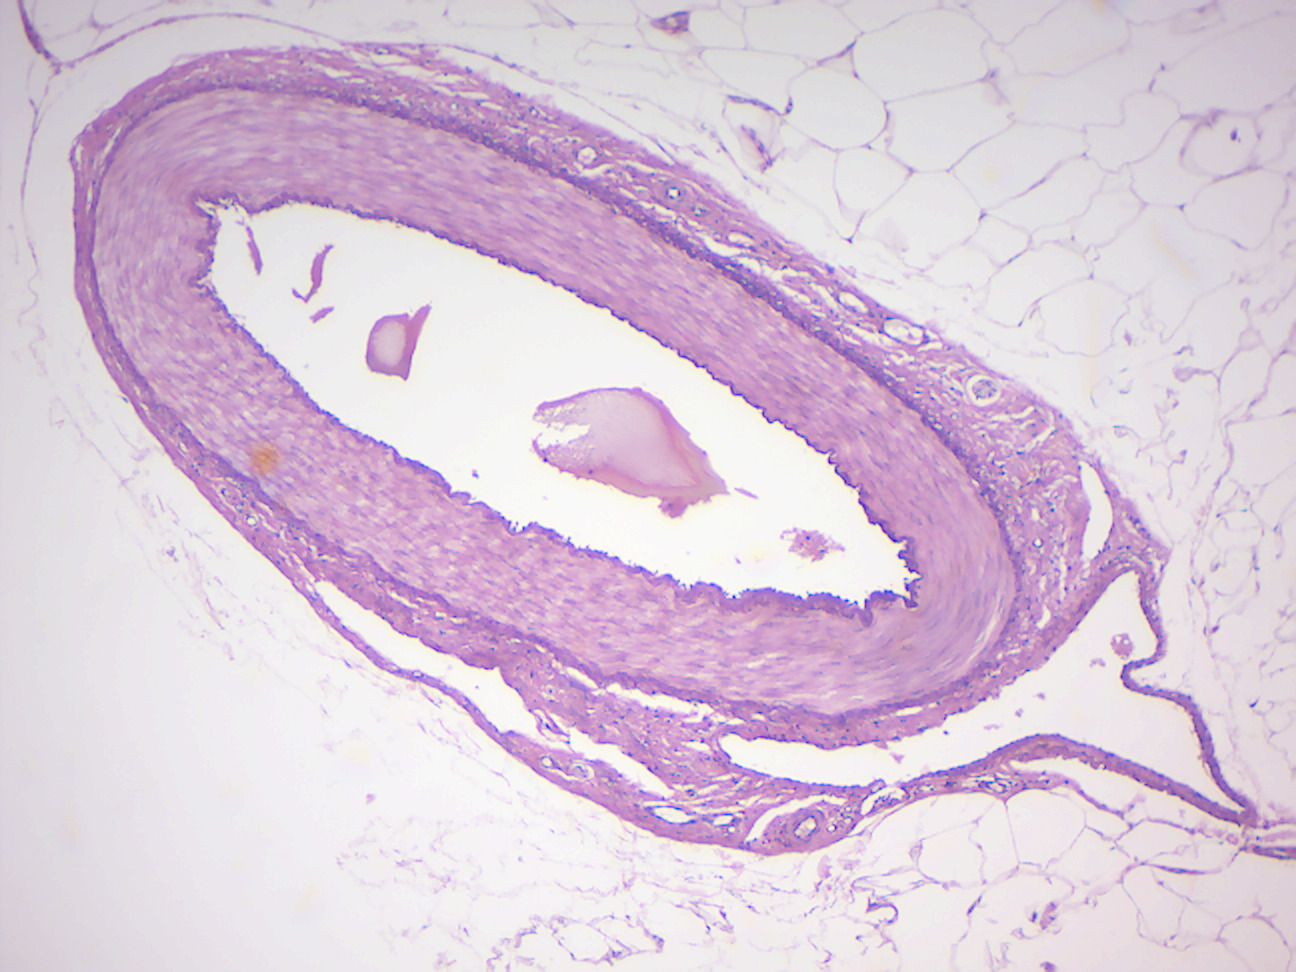
\includegraphics[width=0.7\linewidth]{./figures/anatomy/vessels}

}

\caption{Artery, vein, capillary.}\label{fig:vessels}
\end{figure}

\begin{figure}

{\centering 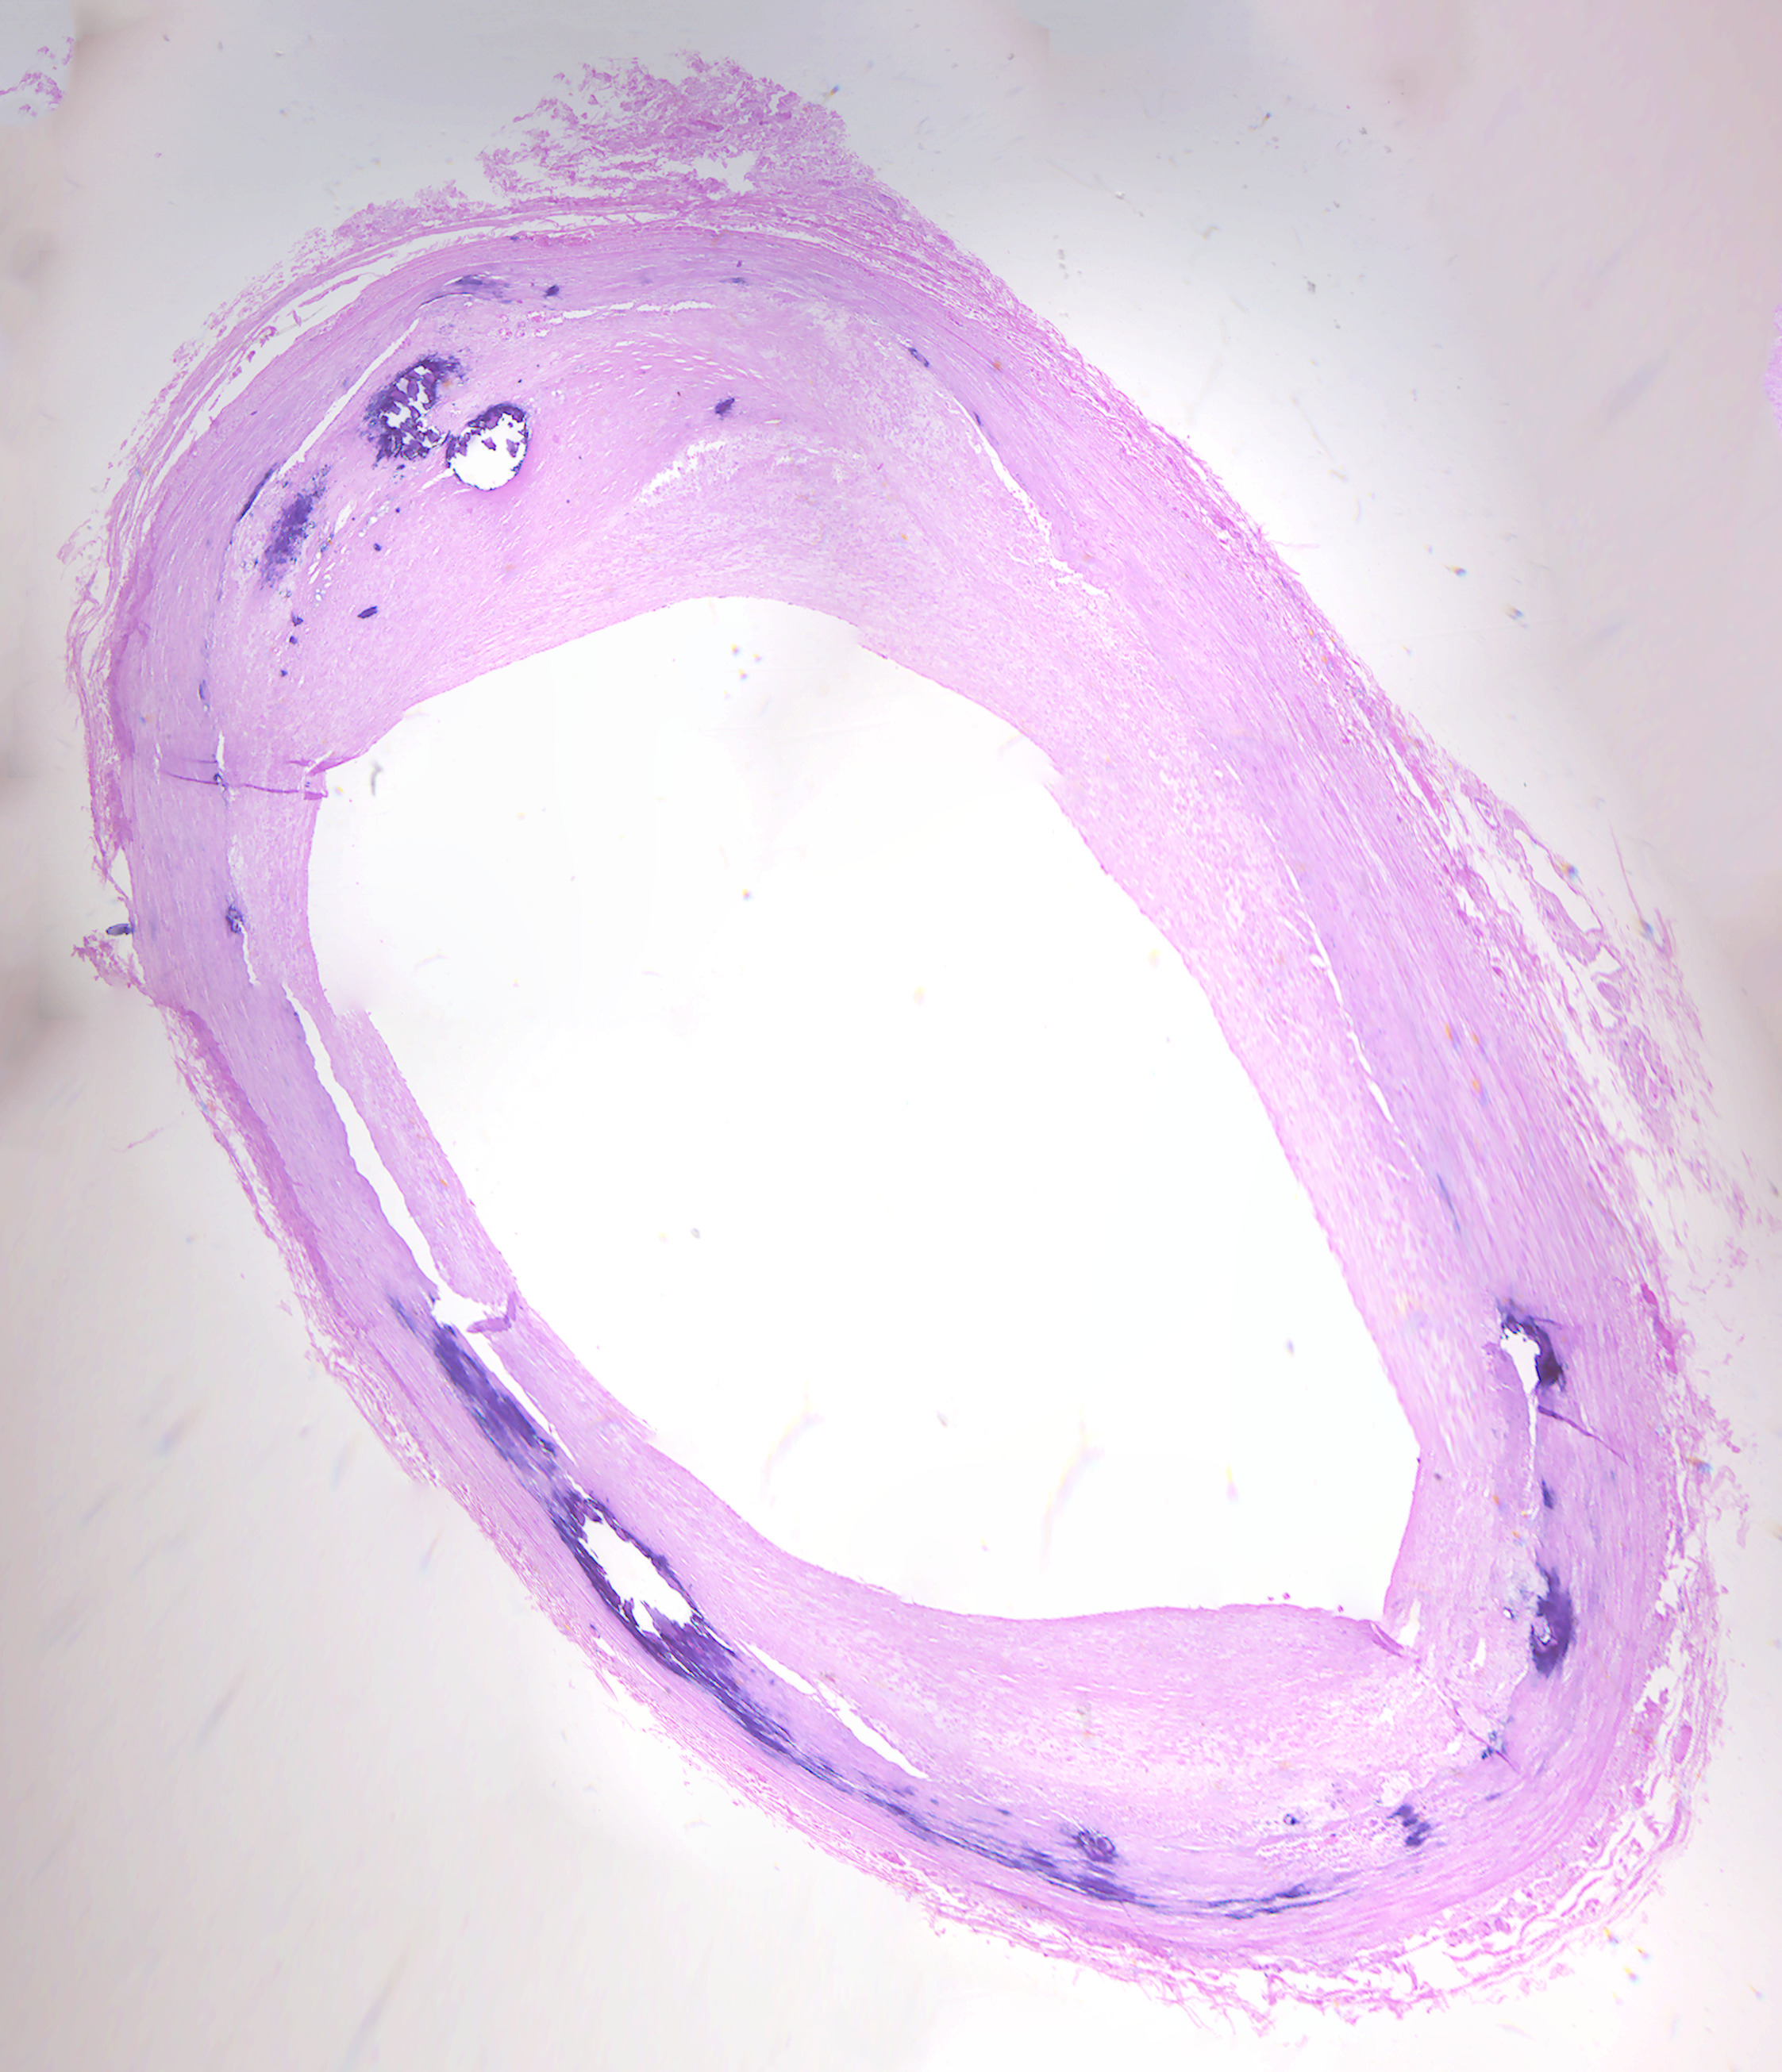
\includegraphics[width=0.7\linewidth]{./figures/anatomy/atherosclerosis}

}

\caption{Atherosclerosis.}\label{fig:atherosclerosis}
\end{figure}

\begin{figure}

{\centering 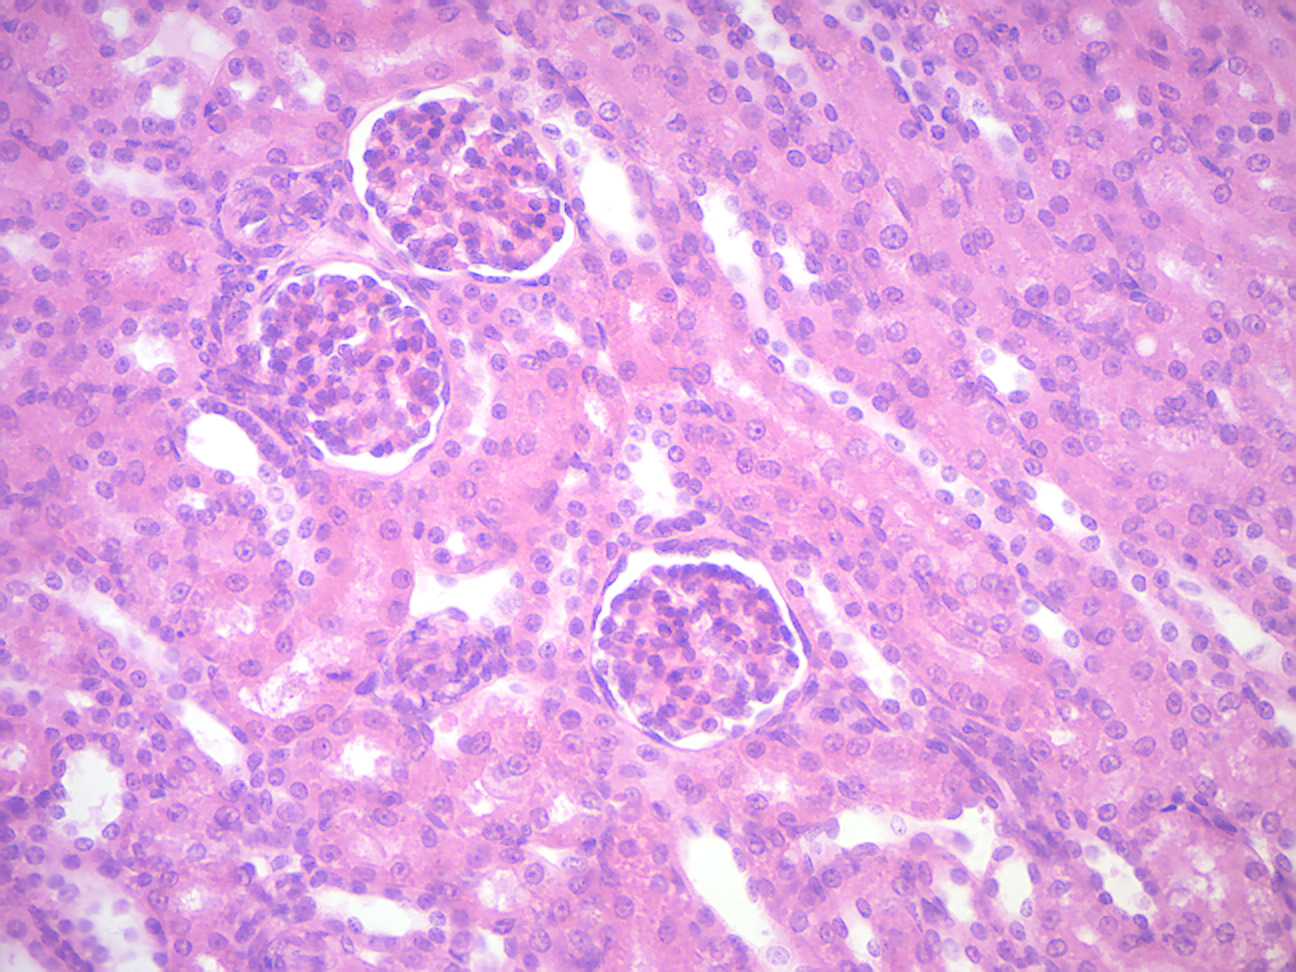
\includegraphics[width=0.7\linewidth]{./figures/anatomy/kidney}

}

\caption{Cortex of the kidney.}\label{fig:kidney}
\end{figure}

In the skin slides listed below identify as many of the following as you
can find:

\begin{itemize}
\tightlist
\item
  skin layers: epidermis, dermis, sub-cutaneous
\item
  blood vessel
\item
  dense fibrous irregular connective tissue
\item
  keratinized layer in epidermis
\item
  adipose tissue
\item
  smooth muscle of pilli
\item
  stratified squamous epithelium
\item
  hair
\item
  hair follicle
\item
  hair root
\item
  hair papilla
\item
  sweat glands
\item
  sebaceous glands
\item
  Vater-Pacini corpuscle
\end{itemize}

\begin{enumerate}
\def\labelenumi{\arabic{enumi}.}
\tightlist
\item
  Unpigmented skin (Figure \ref{fig:unpigmented})
\item
  Axillary skin (Figure \ref{fig:axillary})
\item
  Skin, hairy mammal
\item
  Human scalp hair shafts (Figure \ref{fig:scalp})
\item
  Cornified skin (Figure \ref{fig:cornified})
\item
  Compact Bone (Figure \ref{fig:compactbone})

  \begin{itemize}
  \tightlist
  \item
    Identify: Haversian Systems, osteocytes in lacunae, Haversian Canal,
    canaliculi, calcified matrix
  \end{itemize}
\item
  Bone Ground Human x.s. (Figure \ref{fig:groundbone})

  \begin{itemize}
  \tightlist
  \item
    Identify: Haversian Systems, osteocytes in lacunae, Haversian Canal,
    canaliculi, calcified matrix
  \end{itemize}
\end{enumerate}

\begin{figure}

{\centering 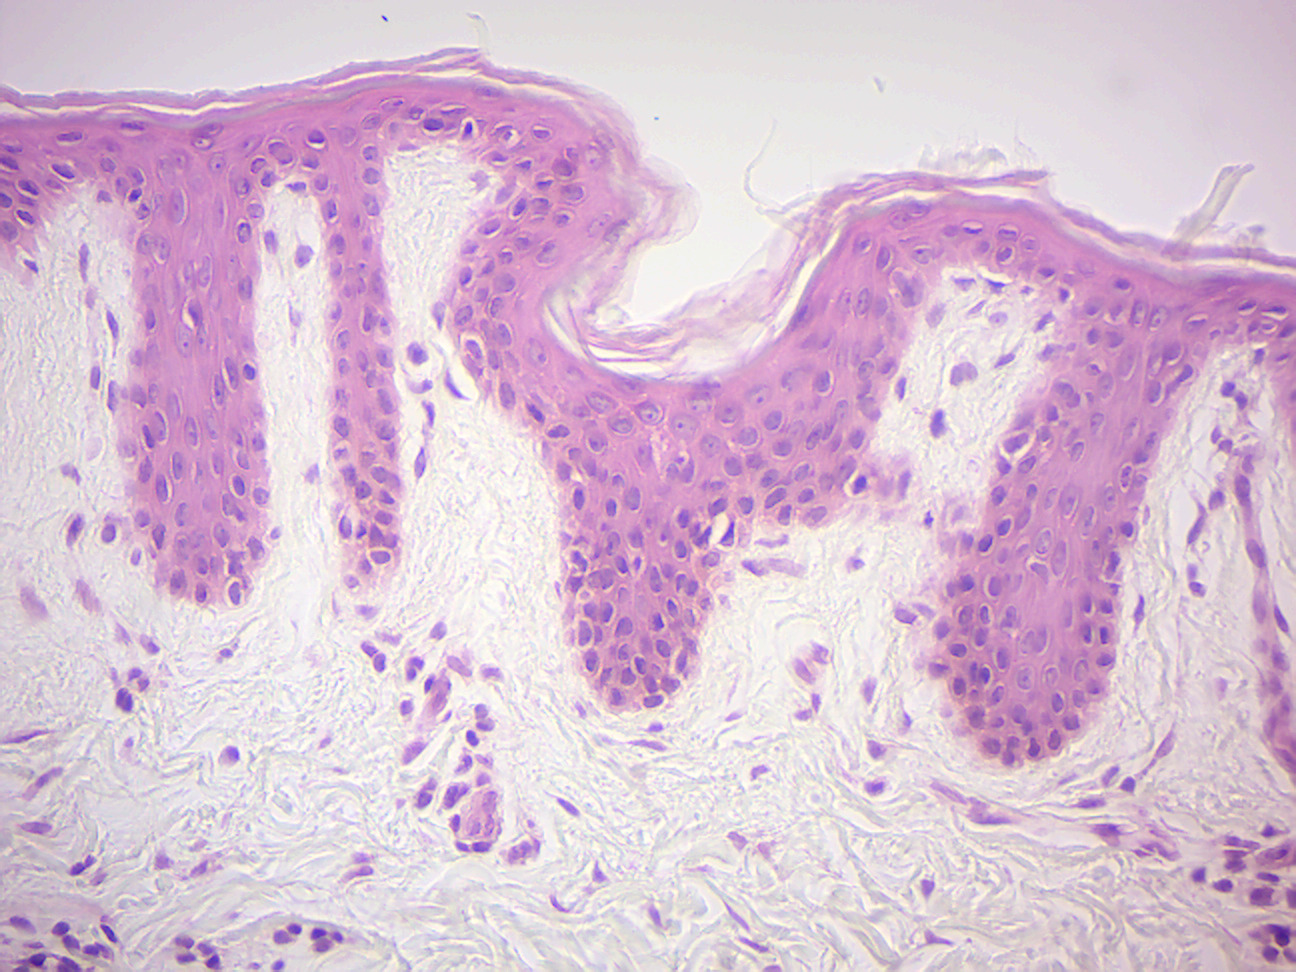
\includegraphics[width=0.7\linewidth]{./figures/anatomy/unpigmented_skin}

}

\caption{Unpigmented skin.}\label{fig:unpigmented}
\end{figure}

\begin{figure}

{\centering 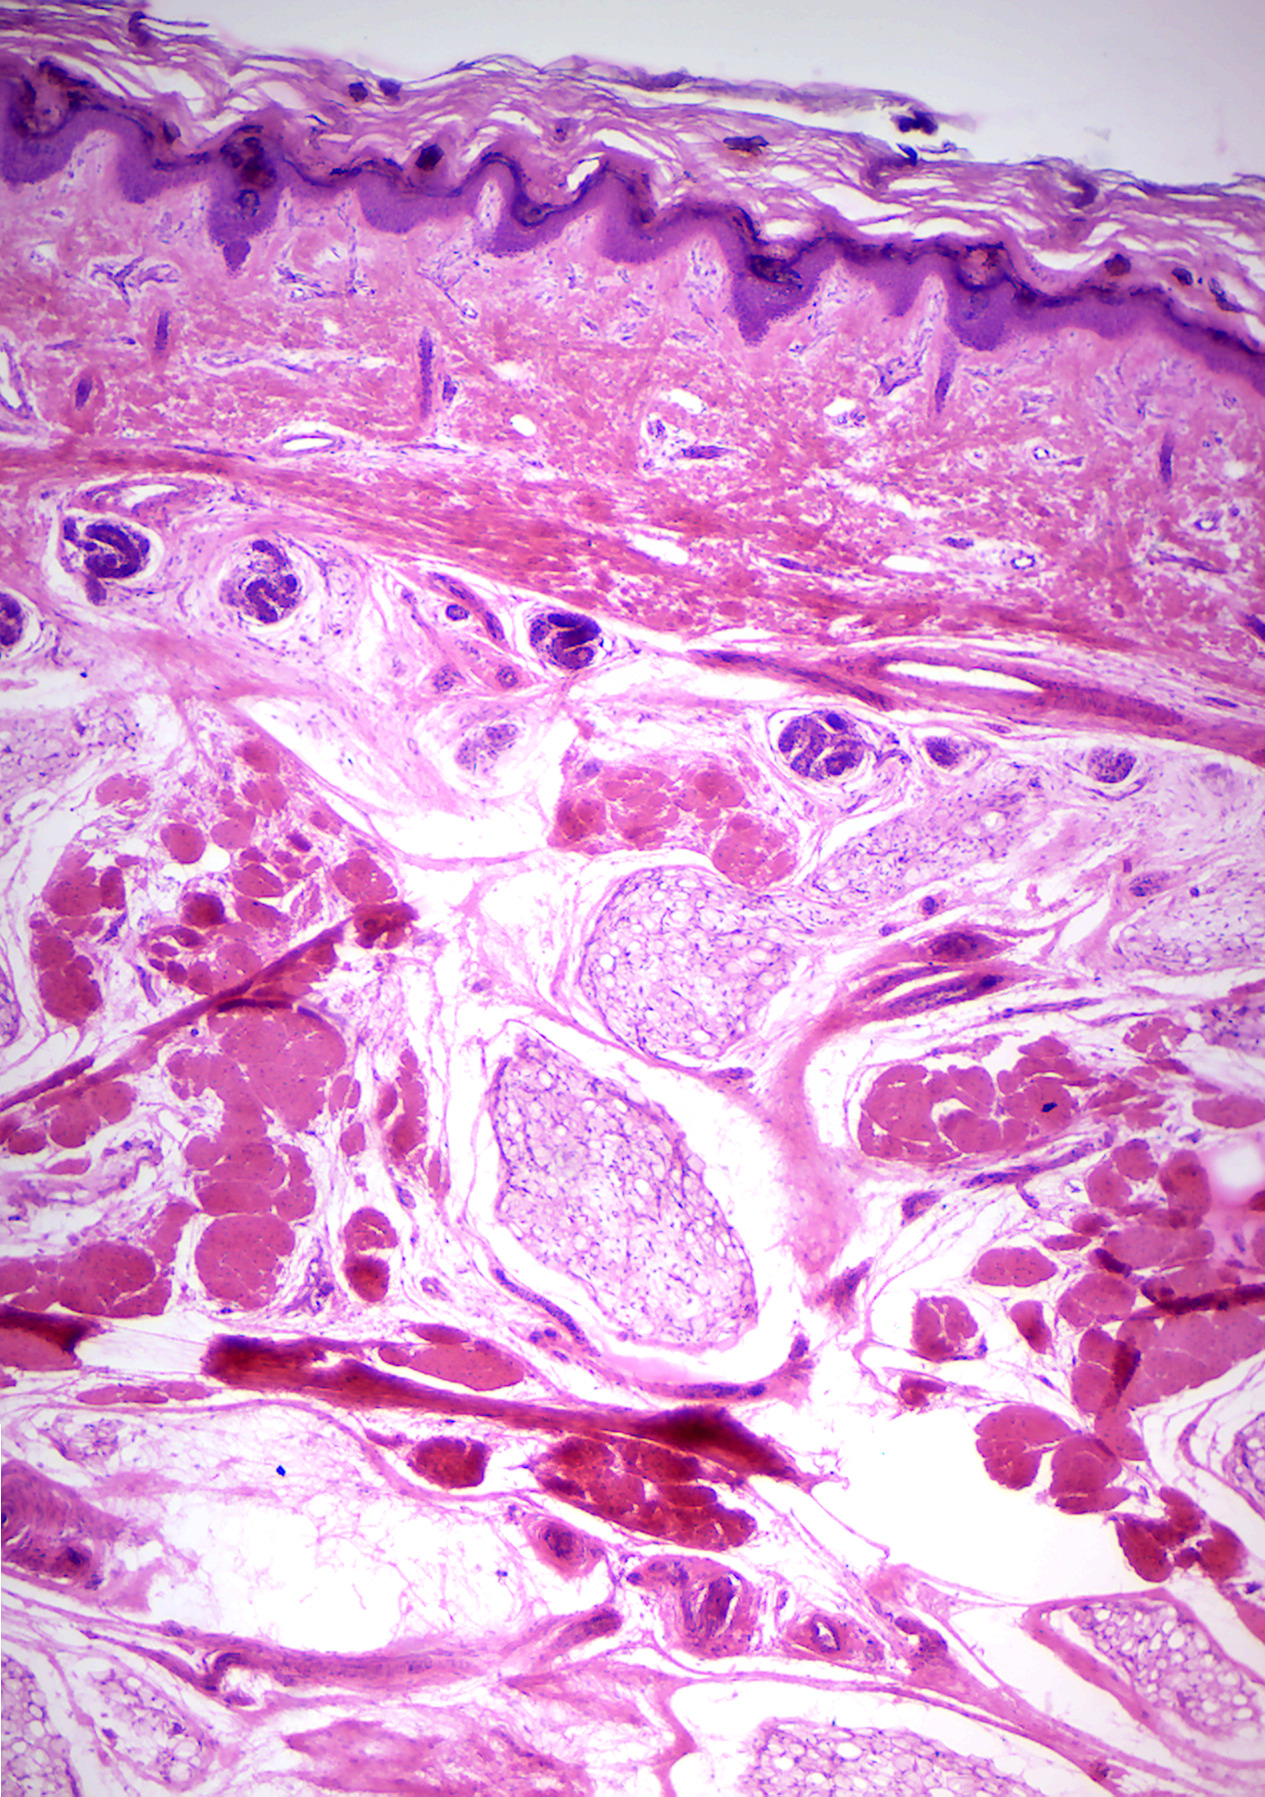
\includegraphics[width=0.7\linewidth]{./figures/anatomy/axillary_skin}

}

\caption{Axillary skin.}\label{fig:axillary}
\end{figure}

\begin{figure}

{\centering 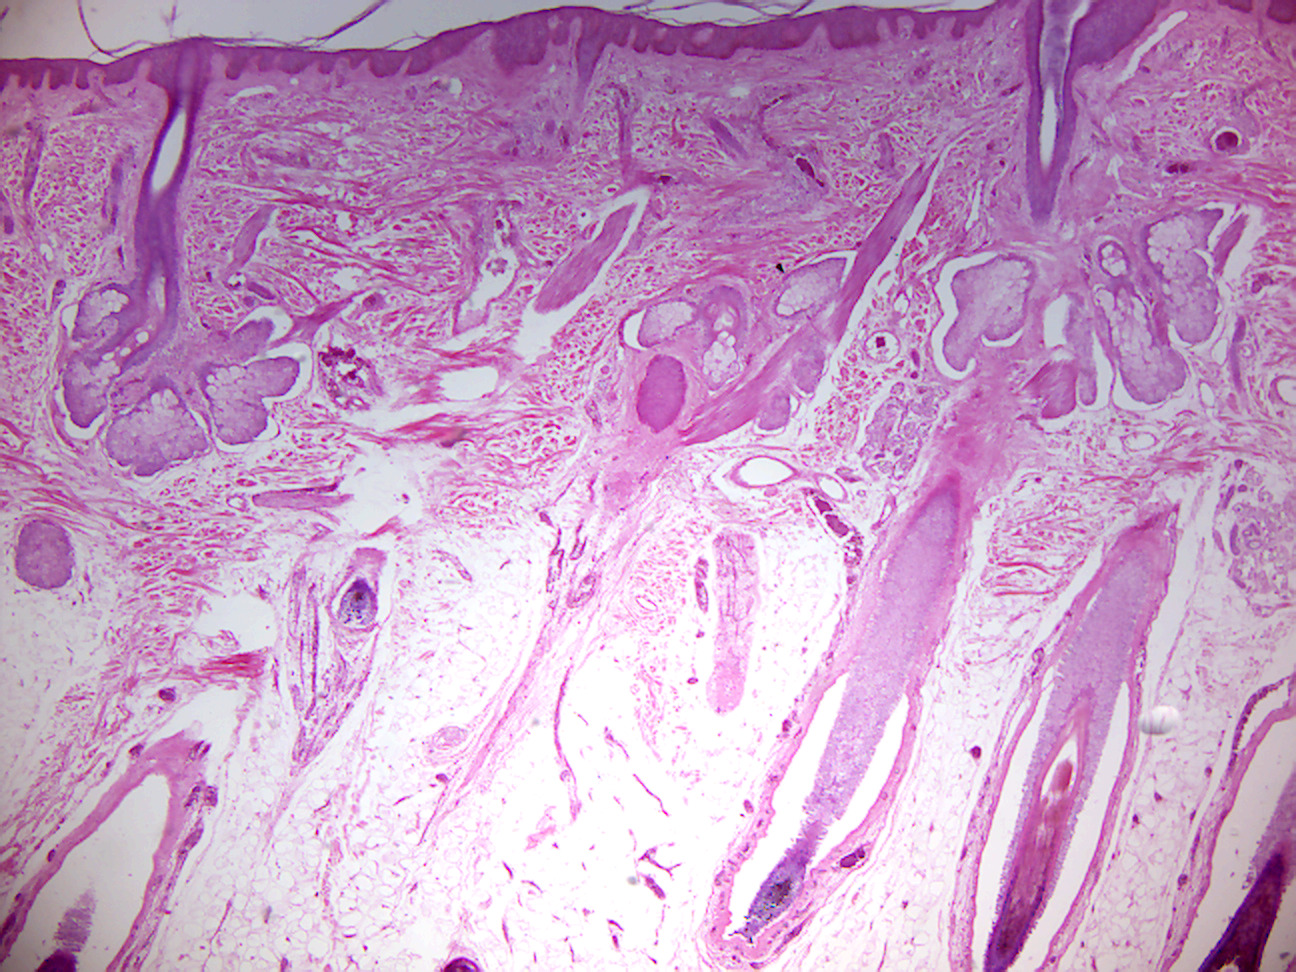
\includegraphics[width=0.7\linewidth]{./figures/anatomy/human_scalp}

}

\caption{Human scalp.}\label{fig:scalp}
\end{figure}

\begin{figure}

{\centering 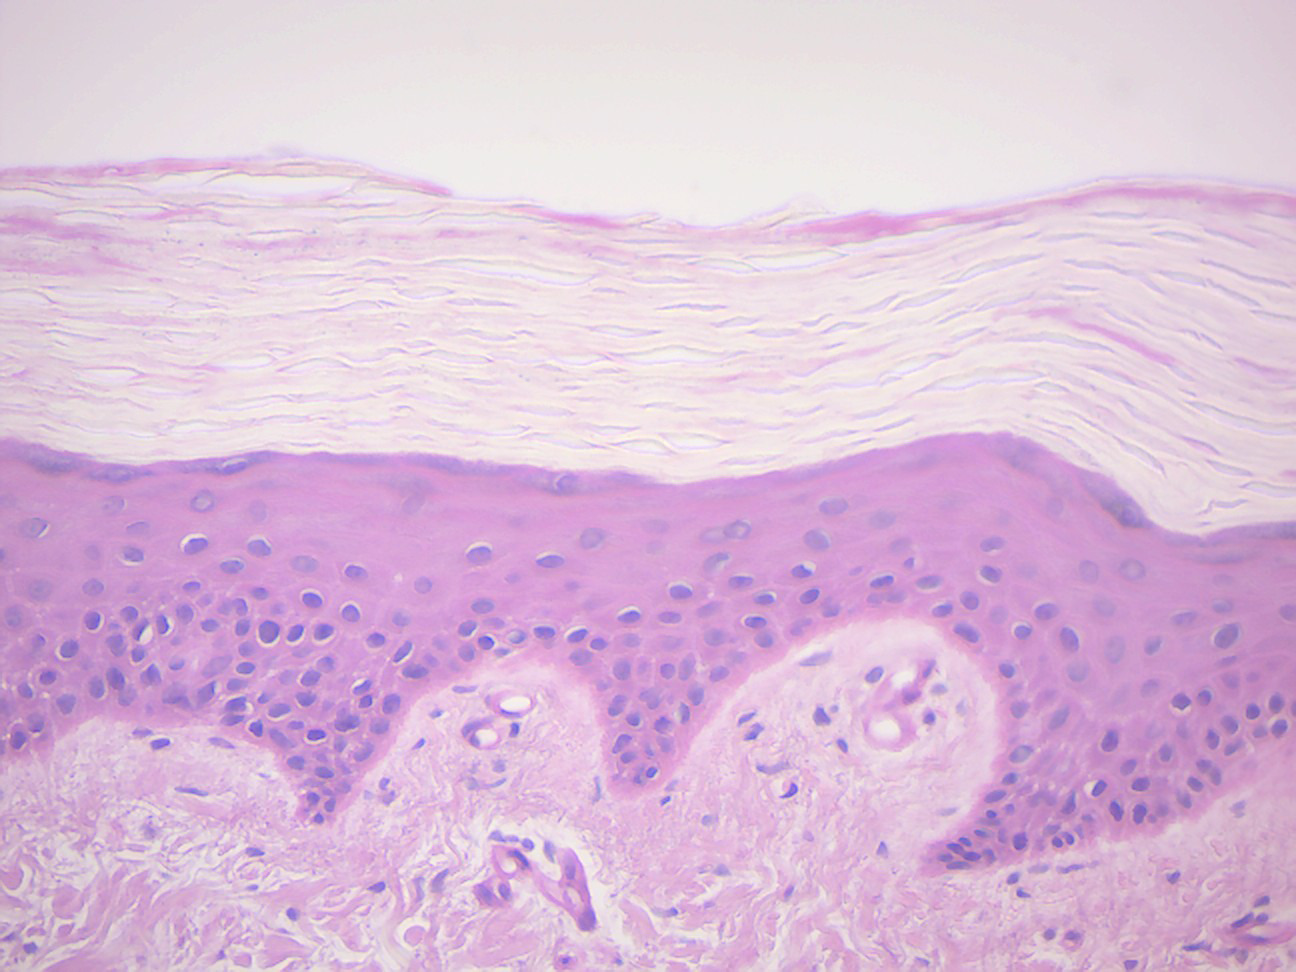
\includegraphics[width=0.7\linewidth]{./figures/anatomy/cornified_skin}

}

\caption{Cornified skin.}\label{fig:cornified}
\end{figure}

\begin{figure}

{\centering 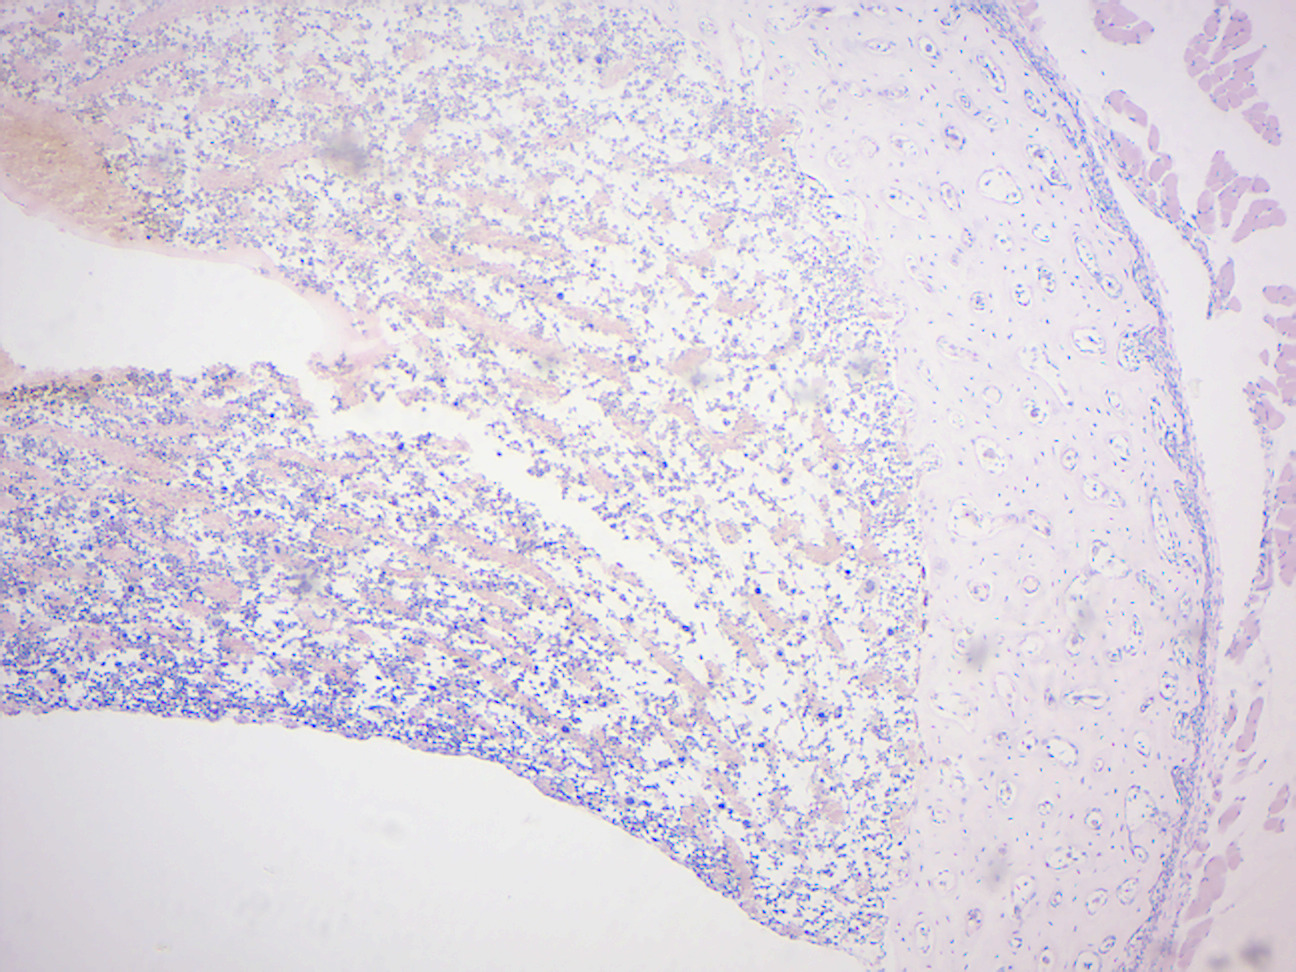
\includegraphics[width=0.7\linewidth]{./figures/anatomy/compact_bone}

}

\caption{Compact Bone.}\label{fig:compactbone}
\end{figure}

\section{The human skeleton}\label{the-human-skeleton}

The \href{https://en.wikipedia.org/wiki/Human_skeleton}{human skeleton}
(Figure \ref{fig:skeleton}) is the internal framework of the body. It is
composed of around 270 bones at birth and around 206 bones by adulthood
after some bones get fused together. The bone mass in the skeleton
reaches maximum density around age 21. The human skeleton can be divided
into the axial skeleton and the appendicular skeleton. The axial
skeleton is formed by the vertebral column, the rib cage, the skull and
other associated bones. The appendicular skeleton, which is attached to
the axial skeleton, is formed by the shoulder girdle, the pelvic girdle
and the bones of the upper and lower limbs.

The human skeleton performs six major functions; support, movement,
protection, production of blood cells, storage of minerals, and
endocrine regulation.

The human skeleton is not as sexually dimorphic as that of many other
primate species, but subtle differences between sexes in the morphology
of the skull, dentition, long bones, and pelvis exist. In general,
female skeletal elements tend to be smaller and less robust than
corresponding male elements within a given population. The human female
pelvis is also different from that of males in order to facilitate
childbirth. Unlike most primates, human males do not have penile bones.

\begin{figure}

{\centering \includegraphics[width=0.7\linewidth]{./figures/anatomy/skeleton}

}

\caption{\href{https://commons.wikimedia.org/wiki/File:Human_skeleton_front_en.svg}{The
human skeleton.}}\label{fig:skeleton}
\end{figure}

\section{Locate the following bones of the human
skeleton:}\label{locate-the-following-bones-of-the-human-skeleton}

\begin{enumerate}
\def\labelenumi{\arabic{enumi}.}
\item
  Axial skeleton:

\begin{verbatim}
Skull Bones:
        Frontal    Mandible
        Parietal   Maxilla
        Temporal   Zygomatic
        Occipital  Nasal

Vertebral Column:
        7 cervical   1 fused sacrum
        12 thoracic  1 fused coccyx
        5 lumbar

    Ribs – 12 pairs; notice the two pairs of “floating” ribs

    Sternum

    Hyoid bone (not shown on small plastic models)
\end{verbatim}
\item
  Appendicular skeleton:

\begin{verbatim}
Pectoral girdle:
      Clavicle  Ulna
      Scapula   Carpals
      Humerus   Metacarpals
      Radius    Phalanges

Pelvic girdle:
      Coccyx    Fibula
      Femur     Tarsals
      Patella   Metatarsals
      Tibia     Phalanges
\end{verbatim}
\item
  Skulls:

  \begin{itemize}
  \item
    Adult: locate the following bones: frontal, occipital, temporal
    parietal, mandible, maxilla, zygomatic, nasal, sphenoid, ethmoid.
    Also locate the immoveable joints known as sutures.
  \item
    Fetal: locate the fontanel (``soft spot'')
  \item
    Female and Male Pelvic Bones: Notice the pubic arch angle and other
    characteristics and determine which are female and which are male.
    Locate the ilium, pubis, and ischium bones. Locate the public
    symphysis (classified as a slightly moveable joint) located between
    the pubic bones.
  \end{itemize}
\end{enumerate}

\section{Comparison of Vertebrate
Skeletons}\label{comparison-of-vertebrate-skeletons}

\begin{enumerate}
\def\labelenumi{\arabic{enumi}.}
\item
  Compare the human skeleton to the following:

\begin{verbatim}
Bony Fish   Bird
Frog        Bat
Snake       Cat
Turtle      Monkey
\end{verbatim}
\item
  Locate the following bones in each skeleton (if possible):

\begin{verbatim}
Humerus   Metacarpals Fibula
Radius    Phalanges   Tarsals
Ulna      Femur       Metatarsals
\end{verbatim}
\end{enumerate}

\section{Review Questions}\label{review-questions-9}

\begin{enumerate}
\def\labelenumi{\arabic{enumi}.}
\tightlist
\item
  Describe the journey of the blood through the heart.
\item
  Heart muscle receives blood from two arteries which arise just above
  the aortic valve. These are the \underline{\phantom{answer}} and the
  \underline{\phantom{answer}}.
\item
  The basic functional unit of the kidney is the
  \underline{\phantom{answer}}.
\item
  The blood is filtered in the \underline{\phantom{answer}} of the kidney.
\item
  The valve between the right atrium and ventricle is called the
  \underline{\phantom{answer}} valve.
\item
  The valve between the left atrium and ventricle is called the
  \underline{\phantom{answer}} valve.
\item
  What is the difference between arteries and veins?
\item
  The most superficial layer of the skin is called the
\underline{\phantom{answer}}.
\item
  The hard, outer layer of bones is composed of cortical bone also
  called \underline{\phantom{answer}} bone.
\item
  \underline{\phantom{answer}} bone tissue is the internal tissue of the
  skeletal bone and is an open cell porous network.  
\end{enumerate}
